\documentclass[11pt]{article}

\usepackage[margin=0.88in]{geometry}
\usepackage{amsmath}
\usepackage{amssymb}
\usepackage{booktabs}
\usepackage{graphicx}
\usepackage{microtype}
\usepackage{array}
\usepackage{longtable}
\usepackage{url}
\usepackage{xcolor}
\usepackage[hidelinks]{hyperref}

\definecolor{resultblue}{HTML}{2F6B9A}
\definecolor{warningorange}{HTML}{D9822B}
\definecolor{passgreen}{HTML}{48794A}
\newcommand{\pass}{\textcolor{passgreen}{\textbf{PASS}}}
\newcommand{\code}[1]{\texttt{#1}}

\title{\textbf{A Frozen Deterministic Arithmetic Unit Inside the
Transformer Stack of a Pretrained Language Model}\\
\large A Preregistered, Causally Intervened 0.5B-Parameter Experiment}
\author{Josiah Wilson\\Independent Researcher}
\date{July 26, 2026}

\begin{document}
\maketitle

\begin{abstract}
Can a pretrained language model contain an exact calculator-like process
inside its repeated transformer stack, rather than merely call a tool or
replace an answer after inference? We wrapped the sixth decoder block of
Qwen2.5-0.5B-Instruct (494,032,768 parameters) with a learned
residual-to-digit encoder, a frozen zero-parameter decimal ripple-carry cell,
and a learned typed-symbol-to-residual decoder. Eighteen unmodified
transformer blocks, the original final normalization, and the tied output head
remained downstream. The pretrained model stayed frozen. The two learned
interfaces contained 18,826 parameters (approximately 0.0038\% of the base);
an equally sized rank-ten residual adapter at the same depth served as the
non-deterministic control. Both were trained only on one- to four-digit
addition. In a frozen three-seed study, the internal deterministic model
answered 450/450 five- to eight-digit primary extrapolation examples, 450/450
nine- to twelve-digit examples, and 225/225 carry-chain examples exactly.
The matched learned control scored 0/450 on both extrapolation splits and
3/225 on carry chains. Learned input encoders recovered 1,575/1,575 operand
registers exactly, and the internal model preserved 300/300 complete base
outputs on ineligible prompts. Disabling the unit reduced primary accuracy
from 450/450 to 0/450. Generation followed deliberately wrong internal states
in 90/90 trials and donor-state substitutions in 39/39. A shared-head logit
lens found a negative mean correct-digit margin before the unit and a positive
margin after every subsequent block; the minimum post-unit mean was +9.80
logits. All eight preregistered criteria passed. The result establishes a
narrow architectural proof: typed exact computation can be inserted inside a
pretrained transformer's repeated block stack and causally control ordinary
autoregressive output after substantial downstream computation. It does not
establish general mathematical understanding, natural-language operation
selection, or a calculator compiled into one ordinary scalar neuron.
\end{abstract}

\section*{Technical summary}

\noindent\textbf{Verdict.} The frozen confirmatory experiment was
\textcolor{passgreen}{\textbf{successful}}: all eight simultaneous criteria
passed without replacing a failed seed or changing the protocol.

\begin{center}
\small
\begin{tabular}{p{0.47\linewidth}rrc}
\toprule
Preregistered criterion & Observed & Threshold & Result\\
\midrule
Mean internal primary-OOD exact match & 100.0\% & $\geq 99.0\%$ & \pass\\
Advantage over parameter-matched control & 100.0 points & $\geq 75.0$ & \pass\\
Mean exact operand-register recovery & 100.0\% & $\geq 99.5\%$ & \pass\\
Token-exact language preservation & 100.0\% & $\geq 99.0\%$ & \pass\\
Wrong-state causal-following rate & 100.0\% & $\geq 95.0\%$ & \pass\\
State-substitution causal-following rate & 100.0\% & $\geq 95.0\%$ & \pass\\
Primary accuracy drop with unit off & 100.0 points & $\geq 80.0$ & \pass\\
Minimum post-unit mean logit margin & $+9.80$ & $>0$ & \pass\\
\bottomrule
\end{tabular}
\end{center}

\noindent The principal finding is not simply that a hard-coded adder returns
correct sums. It is that a learned interface extracted both operands from
block-6 residuals, a frozen cell computed on those predicted typed digits
inside the wrapped layer's forward pass, and a learned residual interface made
that state survive eighteen ordinary downstream blocks. Unit ablation and two
internal-state interventions show that generation causally depended on this
path.

\noindent The claim remains bounded. Input position and operation eligibility
were defined by a strict registered grammar; only digit identity was learned
from residuals. The experiment covered nonnegative integer addition up to
twelve-digit operands, greedy decoding, one model revision, three interface
seeds, and 100 preservation prompts per seed.

\section{Motivation}

Language models generate flexible responses by sampling or maximizing learned
conditional distributions. This makes them useful for open-ended language,
but it also makes facts that admit exact algorithms---such as integer
addition---vulnerable to plausible generation errors. Learned arithmetic
modules and arithmetic-specific training can improve extrapolation
\cite{trask2018,jelassi2023,cho2024}. Program compilation and neural
algorithmic reasoning instead explore how explicit computation can coexist
with neural representations \cite{lindner2023,bounsi2024,saldyt2024}.

Dietz and Klakow's Integrated Gated Calculator (IGC) is the closest prior
integrated-calculator architecture \cite{dietz2025}. It freezes Llama 3.1 8B
and trains learned input/output mappings around a non-differentiable
four-operation calculator, reporting 98--99\% on BIG-Bench Arithmetic. IGC
therefore predates this experiment as evidence for the broad concept. The
question here is narrower: whether a typed unit can be placed after block 6 of
a much smaller pretrained model, survive eighteen downstream transformer
blocks, beat an exactly parameter-matched learned control, and pass direct
internal-state interventions.

The motivating hypothesis, proposed by Josiah Wilson, is that deterministic
processes should sometimes be installed as locked internal structure rather
than approximated anew in every model. A small language model could then learn
how to translate between language/residual representations and the known
process while retaining exact execution. Arithmetic is a useful first test:
its transition rules and correctness criterion are unambiguous, and operand
length provides a direct extrapolation axis. Board games and restricted code
interpreters are natural later domains because they combine deterministic
state transitions with generative planning or explanation.

An earlier experiment connected exact arithmetic to the final residual
immediately before Qwen's tied output head. It achieved perfect primary
arithmetic but failed a 99\% preservation requirement because eligibility
could activate late on quoted commands. That result was both promising and
insufficient: the arithmetic path was output-adjacent, and its scope was not
immutable. The present experiment therefore asks a stricter question:

\begin{quote}
Can predicted operands enter a zero-parameter arithmetic cell inside a real
pretrained transformer's repeated layer stack, can the typed result survive
eighteen subsequent native blocks, and can the system preserve base behavior
outside a deterministically scoped command?
\end{quote}

\section{Architecture}

\subsection{Frozen pretrained model}

The base was \code{Qwen/Qwen2.5-0.5B-Instruct}, revision
\begin{sloppypar}
\code{7ae557604adf67be50417f59c2c2f167def9a775}
\end{sloppypar}
\cite{qwen2024}. It has 494,032,768 parameters, 24 Qwen2 decoder blocks, and
hidden width 896. All pretrained weights were frozen. The original sixth block
was retained but placed inside a wrapper that occupies its real entry in
\code{model.model.layers}. The wrapper preserves the block's calling
signature, attention type, and cache behavior.

\begin{center}
\fbox{\begin{minipage}{0.91\linewidth}
\centering
Blocks 1--5
$\rightarrow$ original block 6
$\rightarrow$ learned residual-to-digit encoder\\
$\rightarrow$ \textbf{frozen typed ripple-carry cell}
$\rightarrow$ learned symbol-to-residual decoder\\
$\rightarrow$ unchanged blocks 7--24
$\rightarrow$ original final RMS norm and tied language-model head
\end{minipage}}
\end{center}

The main condition never writes output logits and never replaces generated
text. Its residual contribution is created after block 6; all eighteen
remaining blocks process it before the usual output head produces tokens.

\subsection{Registered input and immutable scope}

The controlled command was:

\begin{verbatim}
Use the internal addition register. Return only the exact integer.
A = 1 2 3
B = 4 5
\end{verbatim}

Space separation makes every operand digit a stable individual token. A fixed
full-request matcher locates the operand character spans and maps them to
token positions using tokenizer offsets. This locator supplies positions and
length masks but does not read digit values. Quoted, negated, prefixed,
suffixed, documented, or nested versions fail the full match.

Eligibility is decided once before generation and latched immutably for the
response. This is a direct architectural repair of the earlier late-routing
failure. On 1,000 pilot examples with independently sampled one- to
twenty-digit operands, structural recovery was exact in 1,000/1,000 cases and
1,000/1,000 quoted variants were rejected.

\subsection{Learned residual-to-register encoder}

For each structurally selected operand position \(i\), a learned affine
classifier maps the residual after block 6 to a typed digit:

\[
q(h_i)=\arg\max_{d\in\{0,\ldots,9\}} (Wh_i+b)_d,
\qquad
W\in\mathbb{R}^{10\times896}.
\]

The encoder has \(10\cdot896+10=8{,}970\) trainable parameters. It was trained
with supervised digit labels for 300 AdamW steps, batch 512, learning rate
0.01, on residuals from 1,000 one- to four-digit additions. It was then frozen.
At inference, the deterministic cell receives only these predicted digit IDs
and fixed length masks; it never receives ground-truth operands or answers.

Pilot probes at depths 6, 12, 18, and 22 recovered every two-operand register
on 300 examples in each of three length bands through nine to twelve digits.
Depth 6 was selected before confirmation because it left the greatest tested
amount of native computation downstream.

\subsection{Frozen typed arithmetic cell}

The zero-trainable-parameter cell contains immutable tensor lookup buffers for
decimal sum and carry. For digits \(a_j,b_j\) and incoming carry \(c_j\), it
computes

\begin{align}
s_j &= (a_j+b_j+c_j)\bmod 10,\\
c_{j+1} &= \left\lfloor(a_j+b_j+c_j)/10\right\rfloor.
\end{align}

A per-example active-width mask handles unequal operand lengths and prevents
shorter batch rows from accumulating carry during padding columns. Randomized
unit tests included zeros, unequal widths, 18-digit operands, and long carry
chains. The cell emits a typed plan over eleven symbols: decimal digits zero
through nine and end-of-answer.

\subsection{Learned register-to-residual decoder}

An eleven-entry, 896-dimensional codebook maps typed result symbol \(z_t\) to
a residual vector. At the current answer position, the wrapper adds

\[
\Delta h_t = 64\frac{E[z_t]}{\lVert E[z_t]\rVert_2},
\qquad E\in\mathbb{R}^{11\times896}.
\]

The codebook has \(11\cdot896=9{,}856\) trainable parameters. It was optimized
for 120 steps, batch two, learning rate 0.01. Gradients passed through blocks
7--24, the final normalization, and the tied head to the codebook, but none of
those pretrained weights were updated. Generation and all final arithmetic
metrics were free-running and autoregressive; teacher forcing was used only
for interface training.

The combined learned interface therefore has 18,826 parameters, approximately
0.0038\% of the base model. The arithmetic cell itself has none.

\subsection{Parameter-matched learned control}

The central control is a rank-ten bottleneck residual adapter placed after
the same sixth block and active at the same registered answer positions:

\[
\Delta h = W_{\mathrm{up}}\,\sigma(W_{\mathrm{down}}h+b_{\mathrm{down}})
+b_{\mathrm{up}}.
\]

Its projections contain exactly 18,826 trainable parameters, matching the
encoder-plus-codebook budget. It has no typed state or deterministic
transition. For a conservative learning opportunity, it received 1,000
training steps rather than the deterministic decoder's 120. Other controls
were the unchanged frozen base, the trained internal model with its unit
disabled, and direct interventions on the typed internal plan.

\section{Frozen protocol}

\subsection{Pilot separation and source freeze}

Pilot work determined the registered grammar, insertion depth, residual
strength, optimization budgets, causal tests, and preservation set. It was not
pooled into confirmatory estimates. The complete protocol, machine-readable
configuration, runner, and tests were committed before confirmation at
\begin{sloppypar}
\code{a2cf317d42ace613817d3b609b60e245402e3783}.
\end{sloppypar}
The runner recorded canonical configuration SHA-256
\begin{sloppypar}
\code{30a31563834e35edd0bdd635b452866d26611d25f75f646f5f08f6ddd963c261}.
\end{sloppypar}

\subsection{Training and fixed evaluation}

Independent training seeds were 2101, 2203, and 2309. Each produced 1,000
one- to four-digit additions. The internal encoder, internal decoder, and
matched learned control were independently initialized for each seed. The
same seed-specific examples trained both mechanisms.

Evaluation seed 884321 was unused during phase-3 tuning. Every trained seed
was tested on the same:

\begin{itemize}
  \item 150 one- to four-digit in-distribution additions;
  \item 150 five- to eight-digit primary OOD additions;
  \item 150 nine- to twelve-digit long OOD additions;
  \item 75 five- to twelve-digit carry-chain additions;
  \item 100 ineligible preservation prompts;
  \item 30 long-OOD wrong-state interventions;
  \item all 13 available equal-length donor/recipient substitutions;
  \item ten first-answer-symbol downstream traces.
\end{itemize}

Arithmetic used complete sequence-level exact match under greedy generation.
The logical evaluation SHA-256 was
\begin{sloppypar}
\code{d217043d5d20bca4f9aade737ee01d62624f91aadeb6ffea9dfd4233ce606ca3}.
\end{sloppypar}
Training-data hashes for seeds 2101, 2203, and 2309 begin
\code{c94bc23b}, \code{3cd15777}, and \code{e82b7637}, respectively; complete
values are stored in the study manifest.

\subsection{Causal and preservation tests}

\textbf{Unit off} disables the residual write in an otherwise trained wrapper.
If arithmetic performance remains, the deterministic path was not necessary.

\textbf{Wrong state} replaces the first typed result digit with a known
different digit. The output counts as causally following only when the whole
generated sequence equals the intervened plan, not the correct sum.

\textbf{State substitution} installs an equal-length donor's complete typed
result in a recipient example. A match requires the recipient generation to
equal the donor state.

\textbf{Downstream trace} applies the shared final RMS normalization and tied
head as a logit lens to the answer-position residual after block 5, after the
wrapped block 6, and after every subsequent block. It records the correct
first digit's rank and its margin over the strongest alternative.

\textbf{Preservation} compares the wrapped model with an independently loaded
base model on ineligible prompts. Passing an example requires equality of the
entire generated token sequence, not merely semantic similarity.

\subsection{Analysis and success rule}

All eight criteria in the technical summary were required simultaneously.
The primary comparison used paired seed-level internal-minus-control
differences. A 100,000-draw percentile bootstrap resampled the three seed
pairs with replacement using analysis seed 20260726. With three seeds, this
describes observed training-seed sensitivity rather than a broad population.
Every seed and exact count is reported below.

\section{Results}

\subsection{The internal unit was exact on every arithmetic split}

\begin{figure}[ht]
\centering
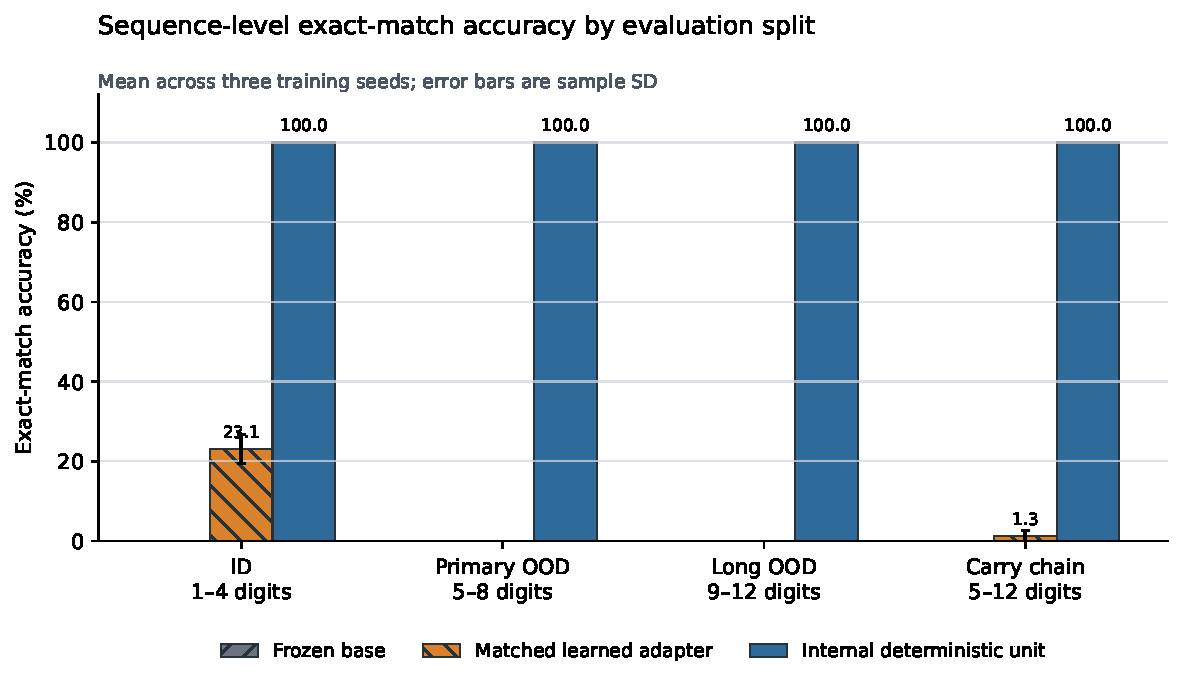
\includegraphics[width=\linewidth]{../phase3_figures/accuracy_by_split.pdf}
\caption{Sequence-level exact match under free-running greedy generation.
Internal and matched-control bars show means over three independently trained
seeds; error bars are sample standard deviations.}
\label{fig:accuracy}
\end{figure}

The internal model answered every one of 1,575 confirmatory arithmetic
examples exactly. This includes 450/450 primary OOD examples, 450/450
nine- to twelve-digit examples, and 225/225 carry-chain examples. The frozen
base scored zero under the controlled exact digit-only response contract and
generally emitted explanatory prose.

\begin{table}[ht]
\centering
\small
\caption{Confirmatory whole-sequence exact match. Parentheses are aggregate
correct/total counts. Internal and learned-control rows pool three seeds; the
frozen base was evaluated once on the fixed sets.}
\label{tab:accuracy}
\begin{tabular}{lrrrr}
\toprule
Condition & ID 1--4 & OOD 5--8 & OOD 9--12 & Carry 5--12\\
\midrule
Frozen base & 0.0\% (0/150) & 0.0\% (0/150) &
0.0\% (0/150) & 0.0\% (0/75)\\
Matched learned adapter & 23.1\% (104/450) & 0.0\% (0/450) &
0.0\% (0/450) & 1.3\% (3/225)\\
Internal deterministic unit & 100.0\% (450/450) & 100.0\% (450/450) &
100.0\% (450/450) & 100.0\% (225/225)\\
\bottomrule
\end{tabular}
\end{table}

\begin{table}[ht]
\centering
\small
\caption{Exact-match accuracy by independently trained seed.}
\label{tab:seeds}
\begin{tabular}{llrrrr}
\toprule
Method & Seed & ID & Primary OOD & Long OOD & Carry\\
\midrule
Internal & 2101 & 100.0\% & 100.0\% & 100.0\% & 100.0\%\\
Internal & 2203 & 100.0\% & 100.0\% & 100.0\% & 100.0\%\\
Internal & 2309 & 100.0\% & 100.0\% & 100.0\% & 100.0\%\\
\midrule
Learned control & 2101 & 26.7\% & 0.0\% & 0.0\% & 0.0\%\\
Learned control & 2203 & 19.3\% & 0.0\% & 0.0\% & 2.7\%\\
Learned control & 2309 & 23.3\% & 0.0\% & 0.0\% & 1.3\%\\
\bottomrule
\end{tabular}
\end{table}

\begin{figure}[ht]
\centering
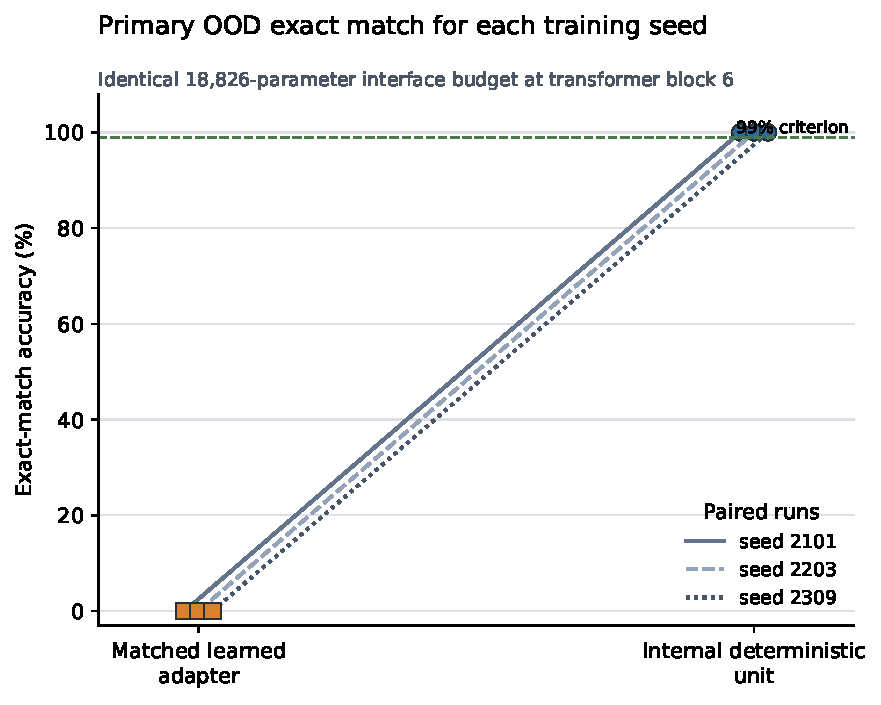
\includegraphics[width=0.78\linewidth]{../phase3_figures/primary_ood_per_seed.pdf}
\caption{Paired primary endpoint. Each line joins the equally sized learned
adapter and internal deterministic unit trained from the same data seed. All
three pairs coincide at a 100-percentage-point difference.}
\label{fig:paired}
\end{figure}

The paired primary difference was 100 percentage points for every seed.
Consequently, the mean was 100 points and the seed-level bootstrap 95\%
percentile interval was [100, 100] points. This degenerate interval is an
honest consequence of identical observed pairs; it should not be interpreted
as eliminating uncertainty outside these three training seeds and this fixed
protocol.

\subsection{The cell consumed correctly decoded internal registers}

Across all four arithmetic splits and three seeds, the frozen learned encoders
recovered both complete operand registers exactly in 1,575/1,575 cases. Mean
primary register accuracy was therefore 100\%, exceeding the 99.5\%
criterion. This rules out a shortcut in which the confirmatory cell receives
ground-truth operand values. The hand-specified locator still provides
positions and widths; the learned classifier provides digit identity.

No internal arithmetic or register errors existed to classify. The matched
learned adapter made \(346+450+450+222=1{,}468\) errors across its 1,575
arithmetic generations. The arithmetic error inventory retains counts by seed
and split.

\subsection{Ablation and interventions establish causal dependence}

With the deterministic unit active, the internal models scored 450/450 on
primary OOD. With the same trained units inactive, they scored 0/450. The
100-point drop exceeds the fixed 80-point requirement.

The stronger tests changed the internal typed plan itself. In 90/90
wrong-state trials, complete free-running generation matched the deliberately
incorrect state. In 39/39 donor substitutions, recipient generation matched
the donor's equal-length plan. These outcomes cannot be explained by a
read-only probe that happens to correlate with an answer: intervening on the
state intervened on the generated result.

\subsection{Exact state remained decodable after eighteen native blocks}

\begin{figure}[ht]
\centering
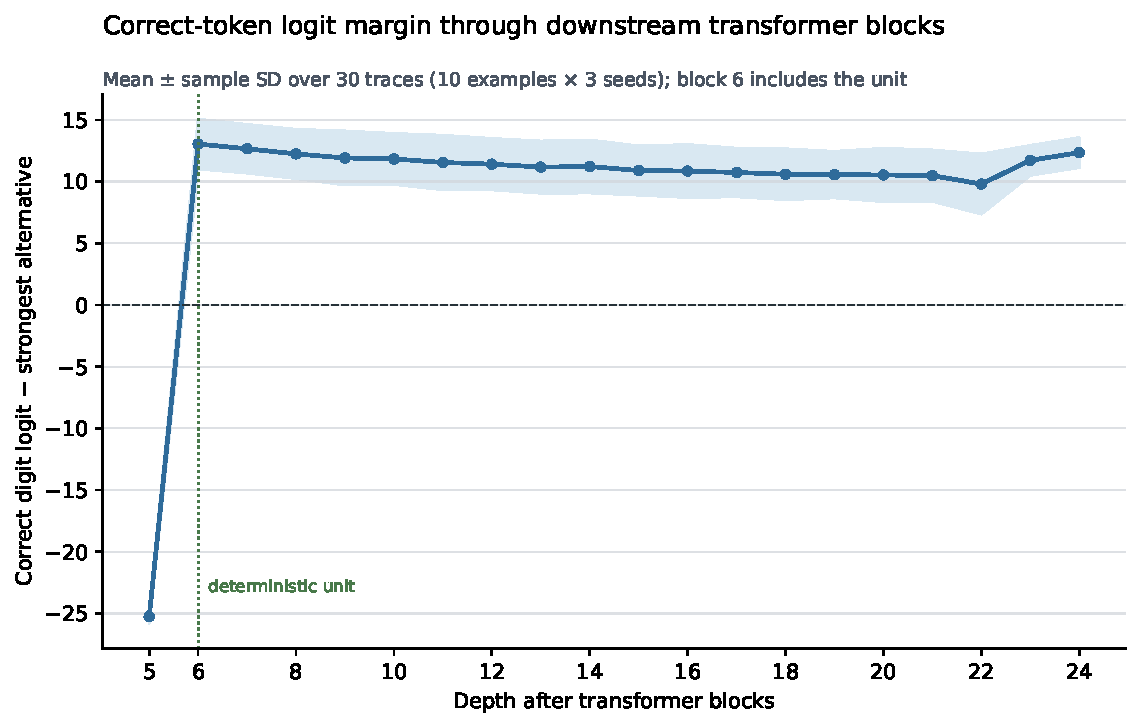
\includegraphics[width=\linewidth]{../phase3_figures/downstream_logit_margin.pdf}
\caption{Correct first-digit logit minus the strongest alternative under a
shared final-normalization/tied-head logit lens. The line is the mean and the
band is sample SD over 30 traces (ten fixed examples times three trained
seeds). Block 6 includes the internal unit.}
\label{fig:trace}
\end{figure}

The mean correct-token margin immediately before the unit, after block 5, was
\(-25.26\) logits; the correct digit was never rank one. After the wrapped
sixth block, the mean margin jumped to \(+13.04\), and the correct digit was
rank one in all 30 traces. The mean remained positive after every downstream
block. Its minimum was \(+9.80\) after block 22; after block 24 it was
\(+12.35\). Even the smallest individual post-unit margin among all traced
depths and examples was positive at \(+5.47\).

This trace does not prove that later blocks manipulate an abstract arithmetic
concept. It shows the narrower property needed here: the unit's answer
representation remained strongly decodable through eighteen ordinary
transformer blocks and the original final head.

\subsection{Deterministic scoping preserved ineligible outputs}

Each trained wrapped model was compared with an independently loaded base on
100 ineligible prompts. These included ordinary questions and valid
register commands embedded in quotes, negations, documentation, prefixes, or
suffixes. All failed full-request eligibility before generation. Complete
generated token sequences matched in 300/300 comparisons.

This repairs the specific earlier failure mode. Eligibility is no longer
searched or re-decided as generation grows; it is a request-level immutable
latch. The test is still small and template-directed. It does not constitute a
general language benchmark or proof against arbitrary adversarial prompting.

\subsection{Training behavior and local feasibility}

Digit-encoder optimization took 0.38--1.65 seconds per seed and reached final
cross-entropy losses from 0.000537 to 0.000594. Internal decoder optimization
took 20.74--36.86 seconds and reached losses from 0.000103 to 0.000137.
The matched learned controls took 160.58--223.67 seconds for 1,000 steps and
ended at losses from 0.500 to 0.847.

These timings are feasibility records rather than a controlled efficiency
claim. The stages have different objectives, batch sizes, step counts, and
device/cache behavior. The full confirmatory archive assembled successfully
on a 16-GiB Apple-silicon computer without remote training compute.

\section{Interpretation}

\subsection{What the experiment demonstrates}

The result supports four linked claims inside the frozen scope:

\begin{enumerate}
  \item digit identity could be read by a small learned classifier from
  intermediate pretrained residuals well beyond training operand lengths;
  \item a zero-parameter exact transition could operate on that predicted
  typed state inside a real transformer-layer wrapper;
  \item a small learned codebook could translate exact typed results back into
  residuals that survived eighteen unmodified blocks;
  \item ordinary generation causally depended on that internal state.
\end{enumerate}

The matched control makes length extrapolation the sharpest distinction.
Equal trainable parameter count, insertion depth, answer positions, training
examples, and downstream model were not enough for an ordinary learned
adapter: it fit 23.1\% of the trained length regime on average and scored zero
on both random extrapolation regimes. The deterministic transition supplied
the correct algorithmic inductive bias.

\subsection{Relation to the proposed ``calculator neuron''}

This experiment is materially closer to the original proposal than an
external tool or output correction. The calculator is a real
\code{torch.nn.Module} executed inside a wrapper occupying one of the 24
repeated layer entries. It consumes values decoded from the model's own
intermediate residuals and returns a residual contribution processed by the
remaining network.

It is not literally one scalar neuron. Decimal addition requires typed
multi-digit state, carry, masks, and translation interfaces. Nor has the
algorithm been compiled into fixed ordinary attention and MLP weights. A
precise name is \emph{an internal deterministic neural-firmware unit with
learned interfaces}. This distinction is not semantic modesty: it identifies
the remaining research question. Future work could ask whether a compiler can
map such a typed process into a fixed differentiable subnetwork or transformer
weights while retaining the same causal and preservation guarantees.

The broad integrated-calculator idea is not new; IGC is direct prior art. The
incremental contribution of this experiment is its deep insertion point,
eighteen-block survival evidence, exactly parameter-matched same-depth
control, learned residual-to-register recovery, and causal wrong-state and
donor-state interventions on a 0.5B model.

\subsection{Why this does not eliminate mathematical hallucination generally}

The system cannot decide whether an arbitrary natural-language problem calls
for addition. It does not parse prose operands, select among operations, prove
theorems, or detect malformed requests. Exact execution begins only after a
strict command envelope and position locator have scoped the task. In a
deployed mathematical assistant, semantic routing and representation would
remain substantial sources of error.

The architectural implication is nevertheless useful: not every component of
mathematical behavior must be entrusted to unconstrained learned generation.
Known subprocedures can be exact even if language understanding around them
remains probabilistic, provided scope, typing, lifetime, and causal integration
are explicit.

\section{Limitations and robustness boundary}

\begin{enumerate}
  \item \textbf{Controlled grammar.} Digits were space separated, operation
  choice was fixed to addition, and a hand-written full matcher supplied token
  positions and operand lengths.
  \item \textbf{One operation and number system.} Only nonnegative base-ten
  integer addition was tested. Signed values, decimals, subtraction,
  multiplication, division, and symbolic mathematics remain untested.
  \item \textbf{Finite length extrapolation.} Training used one to four digits
  and evaluation extended through twelve. The ripple-carry algorithm itself
  is length-generic, but tokenizer context, residual classifiers, generation
  length, and memory impose practical bounds.
  \item \textbf{Small seed count.} Three seeds were sufficient for a frozen
  feasibility test but not for broad estimates across initializations,
  optimizers, hosts, or base models.
  \item \textbf{One pretrained model.} Results may depend on Qwen's tokenizer,
  residual geometry, tied head, and instruction tuning. No Llama-family model
  was tested in this phase.
  \item \textbf{Hard discrete boundary.} Encoder argmax makes the typed cell
  non-differentiable end to end. Staged supervision was intentionally used;
  learning the interface from answer-only loss remains open.
  \item \textbf{Teacher-forced decoder training.} The output codebook was
  trained at known answer positions. Final metrics were free-running, but
  training is easier than unrestricted generation.
  \item \textbf{Matched capacity is not matched computation.} The control has
  equal trainable parameters and location but no explicit typed recurrence.
  It receives more steps; its failure does not establish that every possible
  learned architecture would fail.
  \item \textbf{Preservation scope.} Three hundred exact comparisons cover
  targeted negatives, not general capability retention or all prompt
  injections.
  \item \textbf{Logit-lens interpretation.} Applying the final normalization
  and head at intermediate depths is diagnostic. The causal claims rest on
  ablation and intervention, not the lens alone.
  \item \textbf{Local floating point environment.} MPS kernels and library
  versions may change optimization trajectories. The source, data, model
  revision, hashes, and environment are recorded to enable close replication.
\end{enumerate}

\section{Recommended next experiments}

The next architectural step should widen functionality without weakening the
evidence standard:

\begin{enumerate}
  \item add a typed operation selector and separate frozen cells for
  subtraction and multiplication, while testing deliberately wrong operation
  interventions;
  \item replace the structural token locator with a learned residual-to-register
  extractor over ordinary contiguous numbers, while keeping a separately
  verified scope latch;
  \item repeat on a Llama-class 0.5--1.5B model to test tokenizer and residual
  portability;
  \item compare one internal insertion, repeated shared units, and a fixed
  compiled subnetwork;
  \item train with answer-only supervision using a straight-through or soft
  typed interface, then verify that hard inference remains exact;
  \item test compositional multi-step expressions where the generative model
  chooses and sequences verified primitives;
  \item move to board-game legality/state transition and a restricted
  language parser/type checker as intermediate deterministic domains;
  \item for code, begin with syntax, types, and a sandboxed restricted
  interpreter rather than claiming that open-ended requirements have one
  deterministic correct program.
\end{enumerate}

\section{Reproduction record}

\subsection{Hardware and software}

The study ran locally on Apple arm64 hardware with 16 GiB
(17,179,869,184 bytes) unified memory and MPS available. The operating system
was macOS 26.5.2 build 25F84. The environment used Python 3.12.12,
PyTorch 2.13.0, Transformers 4.57.6, Accelerate 1.14.0,
huggingface-hub 0.36.2, NumPy 2.5.1, Matplotlib 3.11.1, and
safetensors 0.8.0.

The initial frozen launch and final assembly timestamps span 2,274.71 seconds.
A conversation-turn boundary ended the original shell after complete results
for two seeds. Re-running the identical command caused the resumable runner to
skip every completed condition and compute only the unfinished seed-2309
control. Thus the interval includes interruption/resume and is not a pure
throughput benchmark.

\subsection{Commands}

From the frozen source commit:

\begin{verbatim}
git checkout a2cf317d42ace613817d3b609b60e245402e3783
uv sync --extra dev
uv run pytest
uv run ruff check .
uv run python scripts/run_phase3_study.py \
  --config configs/phase3_study.json \
  --artifact-directory phase3_artifacts/confirmatory_v1 \
  --result-directory phase3_results/confirmatory_v1
\end{verbatim}

From the reporting checkout:

\begin{verbatim}
uv run python scripts/analyze_phase3.py
uv run python scripts/hash_phase3_artifacts.py
uv run python scripts/capture_phase3_environment.py
\end{verbatim}

The runner refuses to create a new confirmatory study from dirty source,
records the commit and canonical configuration before fitting, writes a fixed
logical evaluation set, and resumes by retained condition summaries.

\subsection{Artifact inventory}

\begin{longtable}{p{0.40\linewidth}p{0.54\linewidth}}
\toprule
Path & Purpose\\
\midrule
\endhead
\path{PHASE3_PROTOCOL.md} & Human-readable frozen protocol, criteria, and claim
boundary.\\
\path{configs/phase3_study.json} & Machine-readable frozen configuration.\\
\path{PHASE3_LAB_NOTEBOOK.md} & Chronological architecture decisions, pilot
results, caught defects, commands, run/resume record, and confirmatory
outcomes.\\
\path{phase3_results/confirmatory_v1/study.json} & Tracked compact study with
per-example records, seed summaries, hashes, and frozen metadata.\\
\path{phase3_results/confirmatory_v1/analysis.json} & Derived endpoints,
bootstrap, pooled counts, trace criterion, and formal verdict.\\
\path{phase3_results/confirmatory_v1/*.csv} & Accuracy, register, preservation,
intervention, ablation, trace, training, criteria, and error inventories.\\
\path{phase3_results/confirmatory_v1/environment.json} & Model revision,
platform, package, MPS, and source record.\\
\path{phase3_results/confirmatory_v1/artifact_manifest.sha256.json} &
SHA-256 and byte count for every raw local confirmatory file.\\
\path{phase3_figures/} & Reproducible PDF and PNG figures generated only from
the frozen study.\\
\path{phase3_artifacts/confirmatory_v1/} & Local ignored checkpoints, frozen
evaluation, full study, and seed summaries (17 files, 6,410,409 bytes at
reporting time).\\
\path{scripts/run_phase3_study.py} & Resumable confirmatory runner.\\
\path{scripts/analyze_phase3.py} & Deterministic analysis, audit tables,
bootstrap, criteria, and figure generator.\\
\bottomrule
\end{longtable}

\subsection{Audit semantics}

The raw archive manifest stores relative path, byte count, and SHA-256 for all
17 files. Compact records and figures are tracked in Git; checkpoints remain
local under the ignored artifact directory. A portable external archive should
package those raw files with the manifest.

This report separates:

\begin{itemize}
  \item \textbf{pilot}: architecture selection and feasibility evidence not
  included in confirmatory estimates;
  \item \textbf{confirmatory}: the frozen source, configuration, seeds,
  evaluation, and eight-criterion verdict;
  \item \textbf{derived analysis}: deterministic summaries, bootstrap, and
  figures computed after the frozen run.
\end{itemize}

\section{Conclusion}

A zero-parameter exact arithmetic process was successfully installed inside
the repeated block stack of a frozen 494-million-parameter language model.
Learned interfaces totaling 18,826 parameters translated block-6 residuals
into typed operands and typed results back into residuals. The system achieved
1,575/1,575 exact arithmetic generations, including perfect length
extrapolation, while an equally sized learned control scored 0/900 across the
two random OOD splits. It preserved 300/300 ineligible outputs.

The evidence goes beyond end accuracy. The learned input interface recovered
every evaluated register; unit ablation removed the gain; wrong and substituted
states controlled generated answers; and the correct symbol remained
positively decodable after every one of eighteen downstream blocks. All eight
preregistered criteria passed.

The most accurate interpretation is neither ``the LLM learned perfect math''
nor ``a calculator tool fixed the answer afterward.'' A deterministic typed
module ran inside a transformer-layer wrapper and communicated through learned
residual interfaces. This architectural proof supports the broader neural
firmware hypothesis: known exact processes can be embedded within generative
models so that learning handles translation and composition while selected
state transitions remain deterministic. It should be read as a controlled
small-model replication and architectural extension of an existing
integrated-calculator research direction, not a claim of first invention.

\section*{Acknowledgments and Attribution}

Josiah Wilson originated this project's neural-firmware research direction and
specified the internal-transformer architectural question. OpenAI Codex
assisted with literature discovery, experimental design, implementation,
execution, statistical analysis, validation, visualization, and manuscript
drafting under Wilson's direction. All claims remain bounded to the archived
artifacts and observed results.

\begin{thebibliography}{10}

\bibitem{trask2018}
A. Trask, F. Hill, S. Reed, J. Rae, C. Dyer, and P. Blunsom.
\newblock Neural Arithmetic Logic Units.
\newblock \emph{NeurIPS}, 2018.
\newblock \url{https://arxiv.org/abs/1808.00508}.

\bibitem{jelassi2023}
S. Jelassi, S. d'Ascoli, C. Domingo-Enrich, Y. Wu, Y. Li, and F. Charton.
\newblock Length Generalization in Arithmetic Transformers.
\newblock 2023.
\newblock \url{https://arxiv.org/abs/2306.15400}.

\bibitem{cho2024}
H. Cho, J. Cha, P. Awasthi, S. Bhojanapalli, A. Gupta, and C. Yun.
\newblock Position Coupling: Improving Length Generalization of Arithmetic
Transformers Using Task Structure.
\newblock 2024.
\newblock \url{https://arxiv.org/abs/2405.20671}.

\bibitem{lindner2023}
D. Lindner, J. Kramar, S. Farquhar, M. Rahtz, T. McGrath, and V. Mikulik.
\newblock Tracr: Compiled Transformers as a Laboratory for Interpretability.
\newblock \emph{NeurIPS}, 2023.
\newblock \url{https://arxiv.org/abs/2301.05062}.

\bibitem{bounsi2024}
W. Bounsi, B. Ibarz, A. Dudzik, J. Hamrick, L. Markeeva, A. Vitvitskyi,
R. Pascanu, and P. Veli\v{c}kovi\'{c}.
\newblock Transformers Meet Neural Algorithmic Reasoners.
\newblock 2024.
\newblock \url{https://arxiv.org/abs/2406.09308}.

\bibitem{saldyt2024}
L. Saldyt and S. Kambhampati.
\newblock Algorithmic Language Models with Neurally Compiled Libraries.
\newblock 2024.
\newblock \url{https://arxiv.org/abs/2407.04899}.

\bibitem{qwen2024}
Qwen Team.
\newblock Qwen2.5 Technical Report.
\newblock 2024.
\newblock \url{https://arxiv.org/abs/2412.15115}.

\bibitem{hu2021}
E. Hu, Y. Shen, P. Wallis, Z. Allen-Zhu, Y. Li, S. Wang, L. Wang, and W. Chen.
\newblock LoRA: Low-Rank Adaptation of Large Language Models.
\newblock 2021.
\newblock \url{https://arxiv.org/abs/2106.09685}.

\bibitem{vergarabrowne2025}
T. Vergara-Browne and A. Soto.
\newblock Tracr-Injection: Distilling Algorithms into Pre-trained Language
Models.
\newblock 2025.
\newblock \url{https://arxiv.org/abs/2505.10719}.

\bibitem{dietz2025}
F. Dietz and D. Klakow.
\newblock IGC: Integrating a Gated Calculator into an LLM to Solve Arithmetic
Tasks Reliably and Efficiently.
\newblock 2025.
\newblock \url{https://arxiv.org/abs/2501.00684}.

\end{thebibliography}

\end{document}
